\documentclass[11pt, a4paper]{article}

% ── Packages ──────────────────────────────────────────────────────────────────
\usepackage[margin=2.3cm]{geometry}
\usepackage{graphicx}
\usepackage{booktabs}
\usepackage{caption}
\usepackage{subcaption}
\usepackage{amsmath}
\usepackage{float}
\usepackage{array}
\usepackage{xcolor}
\usepackage{multirow}
\usepackage{hyperref}
\usepackage{parskip}
\usepackage{microtype}
\usepackage{enumitem}
\usepackage{longtable}

\graphicspath{{./}}

\hypersetup{colorlinks=true, linkcolor=blue!60!black, citecolor=blue!60!black, urlcolor=blue!60!black}
\captionsetup{font=small, labelfont=bf, skip=6pt}

\definecolor{headblue}{RGB}{21, 101, 192}
\definecolor{lightgray}{RGB}{245, 245, 245}

\title{
    \vspace{-1cm}
    {\Large\textbf{Unsupervised Clustering of Alzheimer's/Dementia Patients}}\\[6pt]
    {\large from Brain MRI and Clinical Data: A Full Pipeline Report}\\[4pt]
    {\normalsize OASIS-1 cross-sectional dataset ($n=416$ patients, $n=216$ complete-case)}
}
\author{Areg Karapetyan}
\date{\today}

\begin{document}
\maketitle
\vspace{-0.4cm}

\begin{abstract}
\noindent This report documents an end-to-end investigation of whether brain-MRI-derived image
features, alone or combined with clinical assessments, can recover clinically meaningful patient
subgroups, specifically groups that align with the Clinical Dementia Rating (CDR) for the
OASIS-1 cross-sectional cohort. Five MRI planes per patient are reduced to per-image PCA components
and combined using a family of robust, mixed-type distance metrics (Robust Mahalanobis, Generalised
Gower, Related Metric Scaling) and a fast $k$-medoids clustering engine. Nine experimental
stages are reported: single-image-type clustering, merged 5-image clustering, clinical+imaging
fusion under Generalised Gower, two-image concatenation, Related Metric Scaling (RelMS), an
image-redundancy correlation analysis, a leave-one-image-out sensitivity sweep, a full
cluster-profiling analysis of the flagship 5-image+clinical configuration, and a per-block
distance-sensitivity study exploiting a package update from the advisor. Across every configuration
tested, the recovered clusters show clear, substantial structure: cluster membership is strongly and
consistently associated with sex (Cram\'er's $V$ up to $0.66$) and total intracranial volume
(eTIV/ASF, $\eta^2$ up to $0.56$), both large effects by conventional standards, and with
education and SES in several configurations. That structure does not, however, align with the
Clinical Dementia Rating (CDR): Adjusted Rand Index (ARI) against CDR stays within roughly
$[-0.02, +0.06]$ and Normalised Mutual Information (NMI) within $[0.01, 0.10]$ throughout, close
to what a random partition would achieve on that axis specifically. Two methodological anomalies
encountered along the way are documented and flagged rather than resolved. Taken together, these
results do not point to an absence of structure in the data. The clustering method works, and works
consistently: it reliably finds real patient groups, just groups organised around demographic and
anatomical variation rather than around dementia severity.
\end{abstract}

\tableofcontents
\newpage

% ══════════════════════════════════════════════════════════════════════════════
\section{Introduction}

Digital/computational pipelines that turn raw, high-dimensional signals (text, images) into a small
set of validated or engineered features, and then cluster those features with a distance metric
suited to mixed data types, are increasingly used across domains. A companion study from the same
advisor (Scielzo-Ortiz, Gran\'e \& D\'iaz-Gorfinkiel, 2026) applies exactly this strategy to Reddit
discourse on the Gaza conflict: LLM-extracted discursive variables (political stance, sentiment,
tone, framing, argument quality) are clustered with a Robust Generalised Gower distance and a fast
$k$-medoids engine, recovering four sociologically interpretable opinion groups and as a key
methodological finding, showing that raw dense text embeddings, used directly as clustering
input, dissolve the very structure the researcher is trying to recover.

This thesis applies the same family of tools to a different domain and a different kind of
high-dimensional input: brain MRI images instead of text. The scientific question is whether
image-derived structural features of the brain, alone or combined with standard clinical
assessments, can recover clinically meaningful patient subgroups for Alzheimer's disease, in
particular, subgroups that line up with the Clinical Dementia Rating (CDR), a standard severity
scale. Unlike the Gaza study, where the validated-feature configuration succeeded and the raw
high-dimensional (embedding) configuration failed, this thesis finds that clustering consistently
succeeds at recovering \emph{some} axis of real patient structure, just not the CDR axis.
Under every combination of image features, clinical features, and distance metric tried, the
clusters produced are large, stable, and strongly differentiated by sex and brain volume (and, in
several configurations, by education and socioeconomic status), but fail to line up with disease
severity. This report documents the full pipeline, methodology, and every experiment run, in order,
together with the figures and numeric results each stage produced, with particular emphasis on
\emph{which} features actually drive each clustering, not only on how well each clustering matches
CDR.

% ══════════════════════════════════════════════════════════════════════════════
\section{Data and Preprocessing}

\subsection{OASIS-1 Dataset}
The Open Access Series of Imaging Studies (OASIS-1) is a cross-sectional collection of 416 subjects
aged 18--96, including cognitively normal individuals and patients with early Alzheimer's disease.
The Clinical Dementia Rating (CDR) is used as the post-hoc evaluation label:
$\mathrm{CDR}=0$ (healthy), $0.5$ (very mild dementia), $1$ (mild dementia), $2$ (moderate dementia).
CDR is known for only 235 of the 416 subjects and is \textbf{never} used as a clustering input;
it is used only to evaluate the clusters after the fact, via Adjusted Rand Index (ARI) and
Normalised Mutual Information (NMI).

\subsection{Five MRI Image Types}
Each patient has up to five MRI planes:
\begin{itemize}[noitemsep]
    \item \texttt{cor}: coronal
    \item \texttt{gfc\_sag}: sagittal, atlas-registered (Talairach space)
    \item \texttt{gfc\_tra}: transverse/axial, atlas-registered
    \item \texttt{masked\_tra}: transverse, brain-masked (non-brain tissue removed)
    \item \texttt{sbj\_sag}: native (subject-space) sagittal, \emph{not} atlas-registered, retains
    individual anatomical variation that registration would otherwise remove
\end{itemize}

\subsection{HOG Feature Extraction}
Each image is padded to a square aspect ratio (centred, zero-padded on the shorter dimension),
resized to $128\times128$ pixels, and converted to Histogram-of-Oriented-Gradients (HOG) features:
9 orientations, $8\times8$ px/cell, $2\times2$ cells/block $\Rightarrow$ \textbf{8{,}100 features per
image}, or \textbf{40{,}500 features per patient} across all five image types.

\subsection{Per-Image PCA}
HOG features are reduced per image type with a two-pass PCA strategy: pass 1 finds, independently
for each image type, the minimum number of components needed to reach 59.2\% explained variance;
the maximum of those minima across the five types (110) is taken as a unified target; pass 2 refits
every image type to exactly 110 components, so all five types are directly comparable
dimensionally. The five resulting $(416\times110)$ PCA matrices are the base feature blocks for
every downstream experiment.

\subsection{Clinical Variables}
Eight clinical variables accompany the imaging features: Age, M/F, Education, Socioeconomic Status
(SES), MMSE (Mini-Mental State Exam), eTIV (estimated total intracranial volume), nWBV (normalised
whole-brain volume), and ASF (atlas scaling factor). Patients missing Education, SES, or MMSE are
dropped (no imputation) for any experiment that uses clinical data, leaving \textbf{216 complete-case
patients}, all of whom have a known CDR.

% ══════════════════════════════════════════════════════════════════════════════
\section{Clustering Methodology}

All clustering uses a family of robust, mixed-type distance metrics and a fast $k$-medoids engine
(\texttt{robust\_mixed\_dist} / \texttt{db\_robust\_clust}, developed by the thesis advisor, Fabio
Scielzo-Ortiz, the same package family used in the Gaza-conflict polarization study referenced
above).

\begin{itemize}[leftmargin=1.4em]
    \item \textbf{Robust Mahalanobis} distance (trimmed, $\alpha=0.05$) for a single quantitative
    block, e.g.\ one image type's 110 PCA components.
    \item \textbf{Generalised Gower (G-Gower)} distance for mixing quantitative, binary, and
    categorical blocks (e.g.\ PCA components + clinical variables) into one distance matrix.
    \item \textbf{Related Metric Scaling (RelMS)}, introduced partway through this project
    specifically to address a block-dominance problem found with G-Gower (Section~\ref{sec:ggower}):
    RelMS treats each declared block (e.g.\ each image type, and the clinical quantitative block)
    \emph{separately}, rescales each by its own geometric variability, and only then combines them,
    so no single block dominates purely because it has more columns.
    \item \textbf{SampleDistClustering / FasterPAM $k$-medoids}: a fast Partitioning-Around-Medoids
    implementation that subsamples for tractability on larger matrices and returns real patients as
    cluster medoids rather than synthetic centroids.
\end{itemize}

\textbf{Evaluation.} Every experiment is evaluated the same way: silhouette score (geometric
separation, computed on all clustered patients), and Adjusted Rand Index (ARI) and Normalised
Mutual Information (NMI) against CDR (computed only on the subset with known CDR). CDR is
multiplied by 2 to obtain integer categories for ARI/NMI. A ``spread'' statistic (the range of
\%~CDR-healthy across clusters) is also tracked as a secondary, more interpretable indicator of
separation. $k \in \{2,3,4\}$ is tested throughout, occasionally up to $k=8$ for formal
$k$-selection diagnostics.

% ══════════════════════════════════════════════════════════════════════════════
\section{Experiments and Results}

Nine experimental stages are reported below, in the order they were run. Two further branches
were also explored but are omitted from this report as exploratory/secondary work: a Tucker
tensor-decomposition alternative to per-image PCA, and a two-stage PCA + Robust Mahalanobis
dimensionality-planning exercise.

\subsection{Single-Image-Type Clustering}

Each of the five image types is clustered on its own 110-component PCA block, with both Euclidean
and Robust Mahalanobis distance, at $k=3$ and $k=4$ (20 combinations total).

\begin{table}[H]
\centering
\footnotesize
\caption{Single-image-type clustering results (20 combinations). Best result overall (highlighted
in the text) is \texttt{masked\_tra}, Euclidean, $k=3$.}
\begin{tabular}{llccccc}
\toprule
\textbf{Image type} & \textbf{Distance} & $k$ & \textbf{Silhouette} & \textbf{ARI} & \textbf{NMI} & \textbf{Spread (\%)} \\
\midrule
Coronal & Euclidean & 3 & 0.0223 & -0.0079 & 0.0221 & 18.4 \\
Coronal & Euclidean & 4 & 0.0079 & -0.0244 & 0.0368 & 31.2 \\
Coronal & Robust Mahalanobis & 3 & 0.0005 & -0.0135 & 0.0127 & 10.0 \\
Coronal & Robust Mahalanobis & 4 & 0.0011 & 0.0094 & 0.0289 & 29.1 \\
Sagittal (atlas) & Euclidean & 3 & 0.0235 & 0.0170 & 0.0189 & 18.8 \\
Sagittal (atlas) & Euclidean & 4 & 0.0210 & 0.0009 & 0.0313 & 19.2 \\
Sagittal (atlas) & Robust Mahalanobis & 3 & 0.0029 & -0.0051 & 0.0070 & 0.9 \\
Sagittal (atlas) & Robust Mahalanobis & 4 & 0.0023 & -0.0014 & 0.0158 & 8.0 \\
Transverse (atlas) & Euclidean & 3 & 0.0009 & -0.0121 & 0.0442 & 33.0 \\
Transverse (atlas) & Euclidean & 4 & 0.0104 & -0.0031 & 0.0485 & 34.7 \\
Transverse (atlas) & Robust Mahalanobis & 3 & 0.0014 & -0.0032 & 0.0124 & 4.8 \\
Transverse (atlas) & Robust Mahalanobis & 4 & 0.0005 & -0.0044 & 0.0097 & 5.3 \\
Masked transverse & Euclidean & 3 & 0.0257 & 0.0597 & 0.0851 & 42.8 \\
Masked transverse & Euclidean & 4 & 0.0062 & 0.0279 & 0.0814 & 47.1 \\
Masked transverse & Robust Mahalanobis & 3 & 0.0004 & -0.0013 & 0.0140 & 10.9 \\
Masked transverse & Robust Mahalanobis & 4 & -0.0001 & 0.0020 & 0.0162 & 14.9 \\
Sagittal (native) & Euclidean & 3 & 0.1348 & -0.0050 & 0.0164 & 12.3 \\
Sagittal (native) & Euclidean & 4 & 0.1112 & -0.0041 & 0.0140 & 13.0 \\
Sagittal (native) & Robust Mahalanobis & 3 & 0.0031 & 0.0060 & 0.0122 & 8.7 \\
Sagittal (native) & Robust Mahalanobis & 4 & -0.0005 & 0.0116 & 0.0187 & 13.9 \\
\bottomrule
\end{tabular}
\end{table}

\noindent The best CDR alignment found anywhere in this entire project comes from this stage:
\texttt{masked\_tra} alone, Euclidean distance, $k=3$ (ARI $=0.060$, NMI $=0.085$). Robust
Mahalanobis performs consistently worse than Euclidean at this stage: most of its ARI values sit
near zero or negative, and silhouette scores collapse to near zero, indicating the robust covariance
estimate is not finding useful structure in a single 110-dimensional PCA block.

\subsection{Merged 5-Image Clustering}

All five image types are concatenated into a single $416\times550$ feature matrix and clustered
with Euclidean and Robust Mahalanobis distance.

\begin{table}[H]
\centering
\caption{Merged 5-image clustering (all 550 PCA features, equal weight per column).}
\begin{tabular}{lcccccc}
\toprule
\textbf{Distance} & $k$ & \textbf{Silhouette} & \textbf{ARI} & \textbf{NMI} & \textbf{Spread (\%)} \\
\midrule
Euclidean & 3 & 0.0371 & -0.0072 & 0.0220 & 9.8 \\
Euclidean & 4 & 0.0366 & 0.0129 & 0.0498 & 33.0 \\
Robust Mahalanobis & 3 & 0.0014 & -0.0006 & 0.0284 & 23.4 \\
Robust Mahalanobis & 4 & -0.0011 & -0.0002 & 0.0342 & 34.5 \\
\bottomrule
\end{tabular}
\end{table}

\noindent Simply merging all five image types performs \emph{worse} than the best single image type
alone (Section 4.1), an early sign that naively concatenating image blocks dilutes rather than
reinforces the signal, motivating the later RelMS approach.

\subsection{Clinical + Imaging Fusion via Generalised Gower}
\label{sec:ggower}

All-5-images-merged PCA features, each single image type's PCA features, and clinical-only
features are each combined with the 8 clinical variables via Generalised Gower distance
(\texttt{SampleDistClustering}, \texttt{metric='ggower'}).

\begin{table}[H]
\centering
\caption{Generalised Gower clustering: condensed view. \textbf{Every} image-type variant
(all-5-merged, each single image type, and even the clinical-only baseline) produced numerically
identical results down to the cluster sizes; three representative rows are shown.}
\begin{tabular}{lcccc}
\toprule
\textbf{Feature set} & $k$ & \textbf{Silhouette} & \textbf{ARI} & \textbf{NMI} \\
\midrule
5 images + clinical & 3 & 0.3272 & 0.0160 & 0.0216 \\
5 images + clinical & 4 & 0.3014 & 0.0006 & 0.0156 \\
Coronal + clinical (representative) & 3 & 0.3284 & 0.0160 & 0.0216 \\
Coronal + clinical (representative) & 4 & 0.3034 & 0.0006 & 0.0156 \\
Clinical only (no imaging) & 3 & 0.3286 & 0.0160 & 0.0216 \\
Clinical only (no imaging) & 4 & 0.3039 & 0.0006 & 0.0156 \\
\bottomrule
\end{tabular}
\end{table}

\noindent \textbf{Anomaly.} This is the first of two methodological anomalies flagged in this
project (see Section~\ref{sec:discussion}). Every image+clinical variant under Generalised Gower,
whether it includes 550, 110, or 0 image PCA columns, produces the \emph{exact same} silhouette,
ARI, NMI, and cluster assignments as the clinical-only baseline. This strongly suggests the clinical
block was dominating the Generalised Gower distance so completely under this particular block
configuration that the image PCA columns contributed essentially zero discriminative signal, most
likely a scaling/normalisation interaction between a 110--550-dimensional quantitative image block
and a 5-dimensional quantitative clinical block within the same distance subspace. This observation
directly motivated switching to RelMS (Section 4.5), which rescales each declared block
independently before combining.

\subsection{Two-Image Concatenation}

As an intermediate step, two image types most likely to be complementary (\texttt{masked\_tra} +
\texttt{cor}) were simply concatenated (Euclidean distance, no explicit block weighting).

\begin{figure}[H]
    \centering
    \includegraphics[width=0.72\textwidth]{elbow_masked_tra_cor_euclidean.png}
    \caption{Elbow curve (FasterPAM loss vs.\ $k$) for the \texttt{masked\_tra}+\texttt{cor}
    concatenated feature matrix, Euclidean distance.}
    \label{fig:elbow_combo}
\end{figure}

\noindent Results stayed near zero (ARI in $[-0.03, 0.01]$ across $k=3,4$), confirming that naive
concatenation, without RelMS-style block rescaling, does not help even for a carefully chosen
pair of image types.

\subsection{Related Metric Scaling (RelMS)}

RelMS treats each image type (and the clinical quantitative variables) as a separate block,
rescaling each by its own geometric variability before combining, specifically to correct the
block-dominance problem found in Section~\ref{sec:ggower}. This was tested on: all 5 images with no
clinical data; all 5 images + clinical (run twice, once with an initial M/F binary/Sokal encoding,
and again after a correction that moved M/F into the multiclass/Hamming block alongside Education
and SES, which is the methodologically correct treatment for a nominal two-category variable); and
the two most promising image pairs, with and without clinical data.

\begin{table}[H]
\centering
\footnotesize
\caption{RelMS results: all-5-image blends, with and without clinical data, before and after the
M/F encoding correction.}
\begin{tabular}{lcccc}
\toprule
\textbf{Configuration} & $k$ & \textbf{Silhouette} & \textbf{ARI} & \textbf{NMI} \\
\midrule
5 images, no clinical & 3 & 0.0183 & -0.0103 & 0.0233 \\
5 images, no clinical & 4 & 0.0106 & -0.0056 & 0.0240 \\
5 images + clinical (initial M/F encoding, $n=216$) & 3 & 0.0159 & 0.0092 & 0.0206 \\
5 images + clinical (initial M/F encoding, $n=216$) & 4 & 0.0112 & 0.0202 & 0.0268 \\
5 images + clinical (corrected M/F encoding, $n=216$) & 2 & 0.0262 & 0.0283 & 0.0107 \\
5 images + clinical (corrected M/F encoding, $n=216$) & 3 & 0.0091 & 0.0176 & 0.0188 \\
\bottomrule
\end{tabular}
\end{table}

\begin{table}[H]
\centering
\footnotesize
\caption{RelMS results: best two-image combinations, with and without clinical data.}
\begin{tabular}{lccccccc}
\toprule
\textbf{Combination} & \textbf{+Clinical} & $k$ & $n$ & \textbf{Silhouette} & \textbf{ARI} & \textbf{NMI} \\
\midrule
masked\_tra+cor & No & 3 & 416 & 0.0068 & -0.0028 & 0.0444 \\
masked\_tra+cor & No & 4 & 416 & 0.0086 & 0.0141 & 0.0437 \\
masked\_tra+gfc\_tra & No & 3 & 416 & 0.0065 & -0.0287 & 0.1009 \\
masked\_tra+gfc\_tra & No & 4 & 416 & 0.0057 & -0.0359 & 0.0624 \\
masked\_tra+cor+clinical & Yes & 3 & 216 & 0.0200 & 0.0323 & 0.0422 \\
masked\_tra+cor+clinical & Yes & 4 & 216 & 0.0138 & 0.0409 & 0.0414 \\
masked\_tra+gfc\_tra+clinical & Yes & 3 & 216 & 0.0203 & 0.0157 & 0.0201 \\
masked\_tra+gfc\_tra+clinical & Yes & 4 & 216 & 0.0138 & 0.0220 & 0.0411 \\
\bottomrule
\end{tabular}
\end{table}

\noindent RelMS moves the numbers slightly upward relative to plain Generalised Gower and simple
concatenation: the best result here, \texttt{masked\_tra+cor+clinical} at $k=4$, reaches
ARI~$=0.041$, NMI~$=0.041$, but still remains far from a meaningful CDR-aligned partition. RelMS fixed
the block-dominance \emph{artifact}, but did not fix the underlying \emph{absence} of CDR-relevant
signal in the image features themselves.

\subsection{Image-Type Redundancy Analysis}

To understand which image types carry unique versus overlapping information, the pairwise-patient
Euclidean distance matrix of each image type (upper triangle, 86{,}320 unique patient pairs) was
correlated against every other image type's distance matrix.

\begin{figure}[H]
    \centering
    \includegraphics[width=0.62\textwidth]{image_correlation_heatmap.png}
    \caption{Pearson correlation between the pairwise-patient-distance matrices of the five image
    types. Higher values mean two image types rank patient similarity almost the same way (redundant);
    lower values mean they capture different structural information (complementary).}
    \label{fig:imgcorr}
\end{figure}

\begin{table}[H]
\centering
\caption{Image-type pairwise distance-matrix correlations, ranked highest to lowest.}
\begin{tabular}{lc}
\toprule
\textbf{Image-type pair} & \textbf{Pearson $r$} \\
\midrule
Coronal $\leftrightarrow$ Sagittal (atlas) & 0.5981 \\
Coronal $\leftrightarrow$ Transverse (atlas) & 0.5735 \\
Sagittal (atlas) $\leftrightarrow$ Transverse (atlas) & 0.4957 \\
Transverse (atlas) $\leftrightarrow$ Masked transverse & 0.4474 \\
Coronal $\leftrightarrow$ Masked transverse & 0.3808 \\
Sagittal (atlas) $\leftrightarrow$ Masked transverse & 0.3158 \\
Sagittal (atlas) $\leftrightarrow$ Sagittal (native) & 0.2132 \\
Transverse (atlas) $\leftrightarrow$ Sagittal (native) & 0.1974 \\
Coronal $\leftrightarrow$ Sagittal (native) & 0.1374 \\
Masked transverse $\leftrightarrow$ Sagittal (native) & 0.0161 \\
\bottomrule
\end{tabular}
\end{table}

\noindent The most redundant pair is \texttt{cor}~$\leftrightarrow$~\texttt{gfc\_sag} ($r=0.598$);
the most complementary/independent pair is \texttt{masked\_tra}~$\leftrightarrow$~\texttt{sbj\_sag}
($r=0.016$), meaning the native (unregistered) sagittal images carry the most anatomically unique
signal, distinct from every other type. This finding directly motivated which image pairs were
prioritised in Section 4.5 and which single blocks were targeted in the per-block distance
sensitivity study (Section 4.9).

\subsection{Leave-One-Image-Out Sweep}

Building on the redundancy finding above, each image type was removed in turn from the RelMS
5-image blend to see whether it was contributing real CDR-relevant signal or mostly noise.

\begin{table}[H]
\centering
\caption{Leave-one-image-out: mean change in ARI/NMI (vs.\ the full 5-image RelMS baseline) across
$k=3,4$, when the named image type is removed. Positive $=$ removing that image \emph{improved}
CDR alignment (it was diluting signal); negative $=$ removing it \emph{hurt} alignment (it was
contributing real signal).}
\begin{tabular}{lcc}
\toprule
\textbf{Image type removed} & \textbf{Mean $\Delta$ARI} & \textbf{Mean $\Delta$NMI} \\
\midrule
Masked transverse & +0.0046 & +0.0050 \\
Coronal & +0.0009 & -0.0128 \\
Sagittal (native) & +0.0003 & +0.0046 \\
Sagittal (atlas) & -0.0050 & -0.0011 \\
Transverse (atlas) & -0.0074 & -0.0010 \\
\bottomrule
\end{tabular}
\end{table}

\noindent Removing \texttt{masked\_tra} or \texttt{sbj\_sag} tends to help slightly, while removing
\texttt{gfc\_sag} or \texttt{gfc\_tra} tends to hurt, consistent with the redundancy finding
(\texttt{gfc\_sag}/\texttt{gfc\_tra} correlate strongly with \texttt{cor} and contribute mostly
overlapping signal, whereas \texttt{masked\_tra}/\texttt{sbj\_sag} are more independent but also
noisier for this task). All deltas, however, are small ($|\Delta\mathrm{ARI}| \leq 0.007$), well
within the noise floor observed throughout this project.

\subsection{Flagship Experiment: Full Cluster Profiling (5 Images + Clinical, RelMS)}
\label{sec:flagship}

The corrected RelMS 5-image+clinical configuration ($n=216$, 558 features: 5$\times$110 image PCA
+ 5 clinical quantitative + 3 clinical categorical) was profiled in the most depth: cluster-by-cluster
clinical/demographic breakdowns, effect-size rankings of which features actually separate the
clusters, and (secondarily) optimal-$k$ selection and geometric separation diagnostics. The emphasis
here is deliberately on \emph{what the clusters are made of}, which features differ between them
and by how much, rather than on clustering-quality scores alone.

\begin{figure}[H]
    \centering
    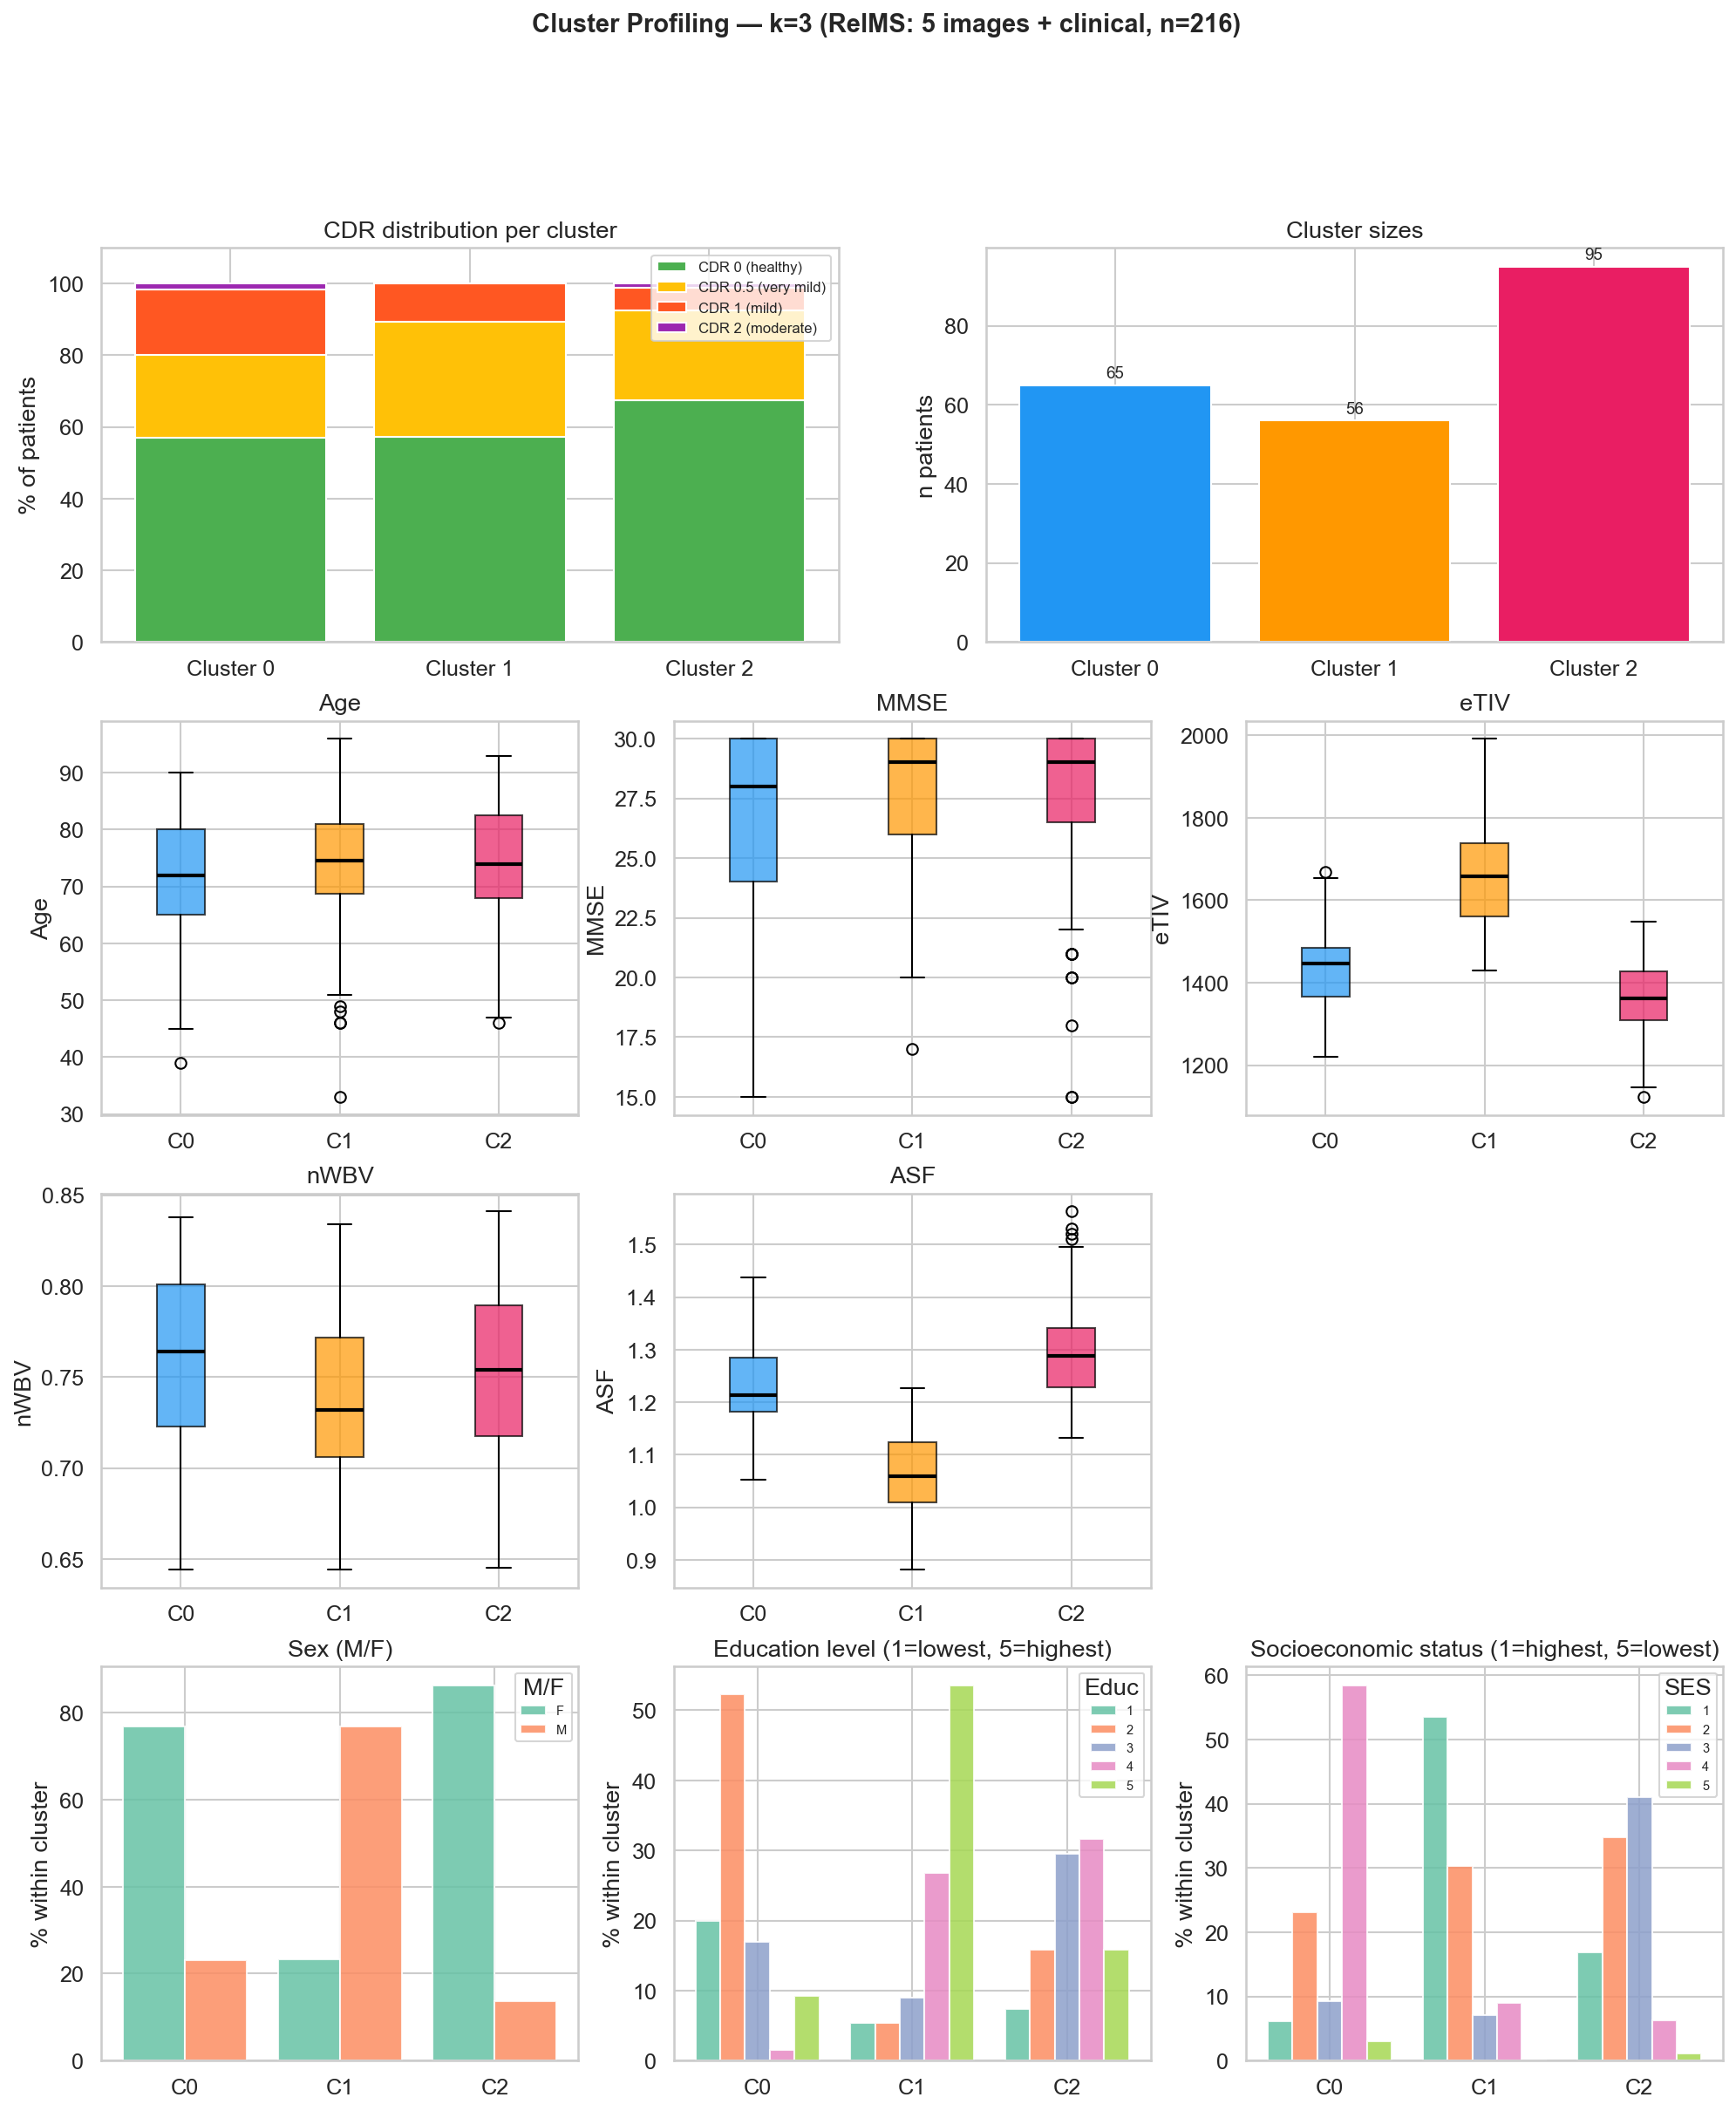
\includegraphics[width=\textwidth]{cluster_profile_k3.png}
    \caption{Full cluster profile at $k=3$: CDR distribution and cluster sizes (top row), boxplots of
    Age, MMSE, eTIV, nWBV and ASF (middle rows), and categorical breakdowns of sex, education and SES
    (bottom row). Sex and eTIV visibly separate the three clusters; CDR, Age and MMSE do not.}
    \label{fig:profilek3}
\end{figure}

\begin{table}[H]
\centering
\footnotesize
\caption{Cluster profiles at $k=3$, 5 images + clinical, RelMS, $n=216$.}
\begin{tabular}{lccccccccccc}
\toprule
\textbf{Cluster} & $n$ & \textbf{CDR0} & \textbf{CDR0.5} & \textbf{CDR1} & \textbf{CDR2} & \textbf{Age} &
\textbf{MMSE} & \textbf{eTIV} & \textbf{Educ} & \textbf{SES} & \textbf{\%F} \\
\midrule
C0 & 65 & 56.9 & 23.1 & 18.5 & 1.5 & 71.3 & 26.75 & 1430 & 2.28 & 3.29 & 76.9 \\
C1 & 56 & 57.1 & 32.1 & 10.7 & 0.0 & 72.4 & 27.62 & 1661 & 4.18 & 1.71 & 23.2 \\
C2 & 95 & 67.4 & 25.3 & 6.3 & 1.1 & 73.2 & 27.54 & 1359 & 3.33 & 2.40 & 86.3 \\
\bottomrule
\end{tabular}
\end{table}

\begin{figure}[H]
    \centering
    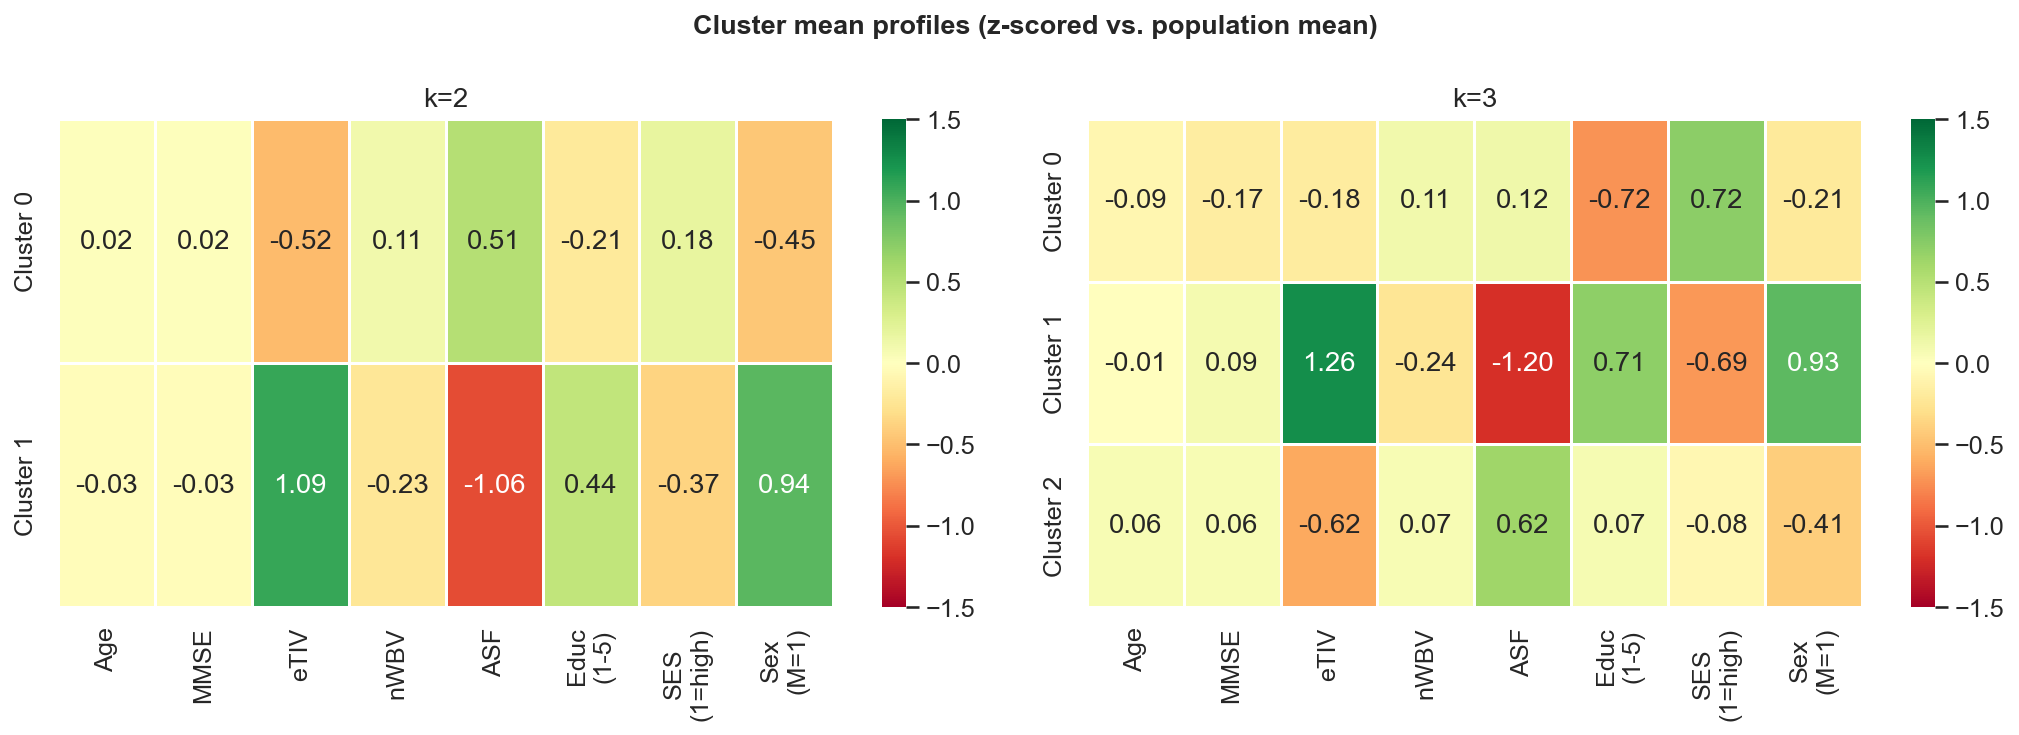
\includegraphics[width=0.85\textwidth]{cluster_profile_heatmap.png}
    \caption{Cluster mean profile (z-scored vs.\ population mean), $k=2$ and $k=3$. Cells further
    from zero indicate a feature on which that cluster deviates most from the overall population.
    Sex (M/F) and eTIV are consistently the strongest differentiators.}
    \label{fig:heatmap18}
\end{figure}

\begin{figure}[H]
    \centering
    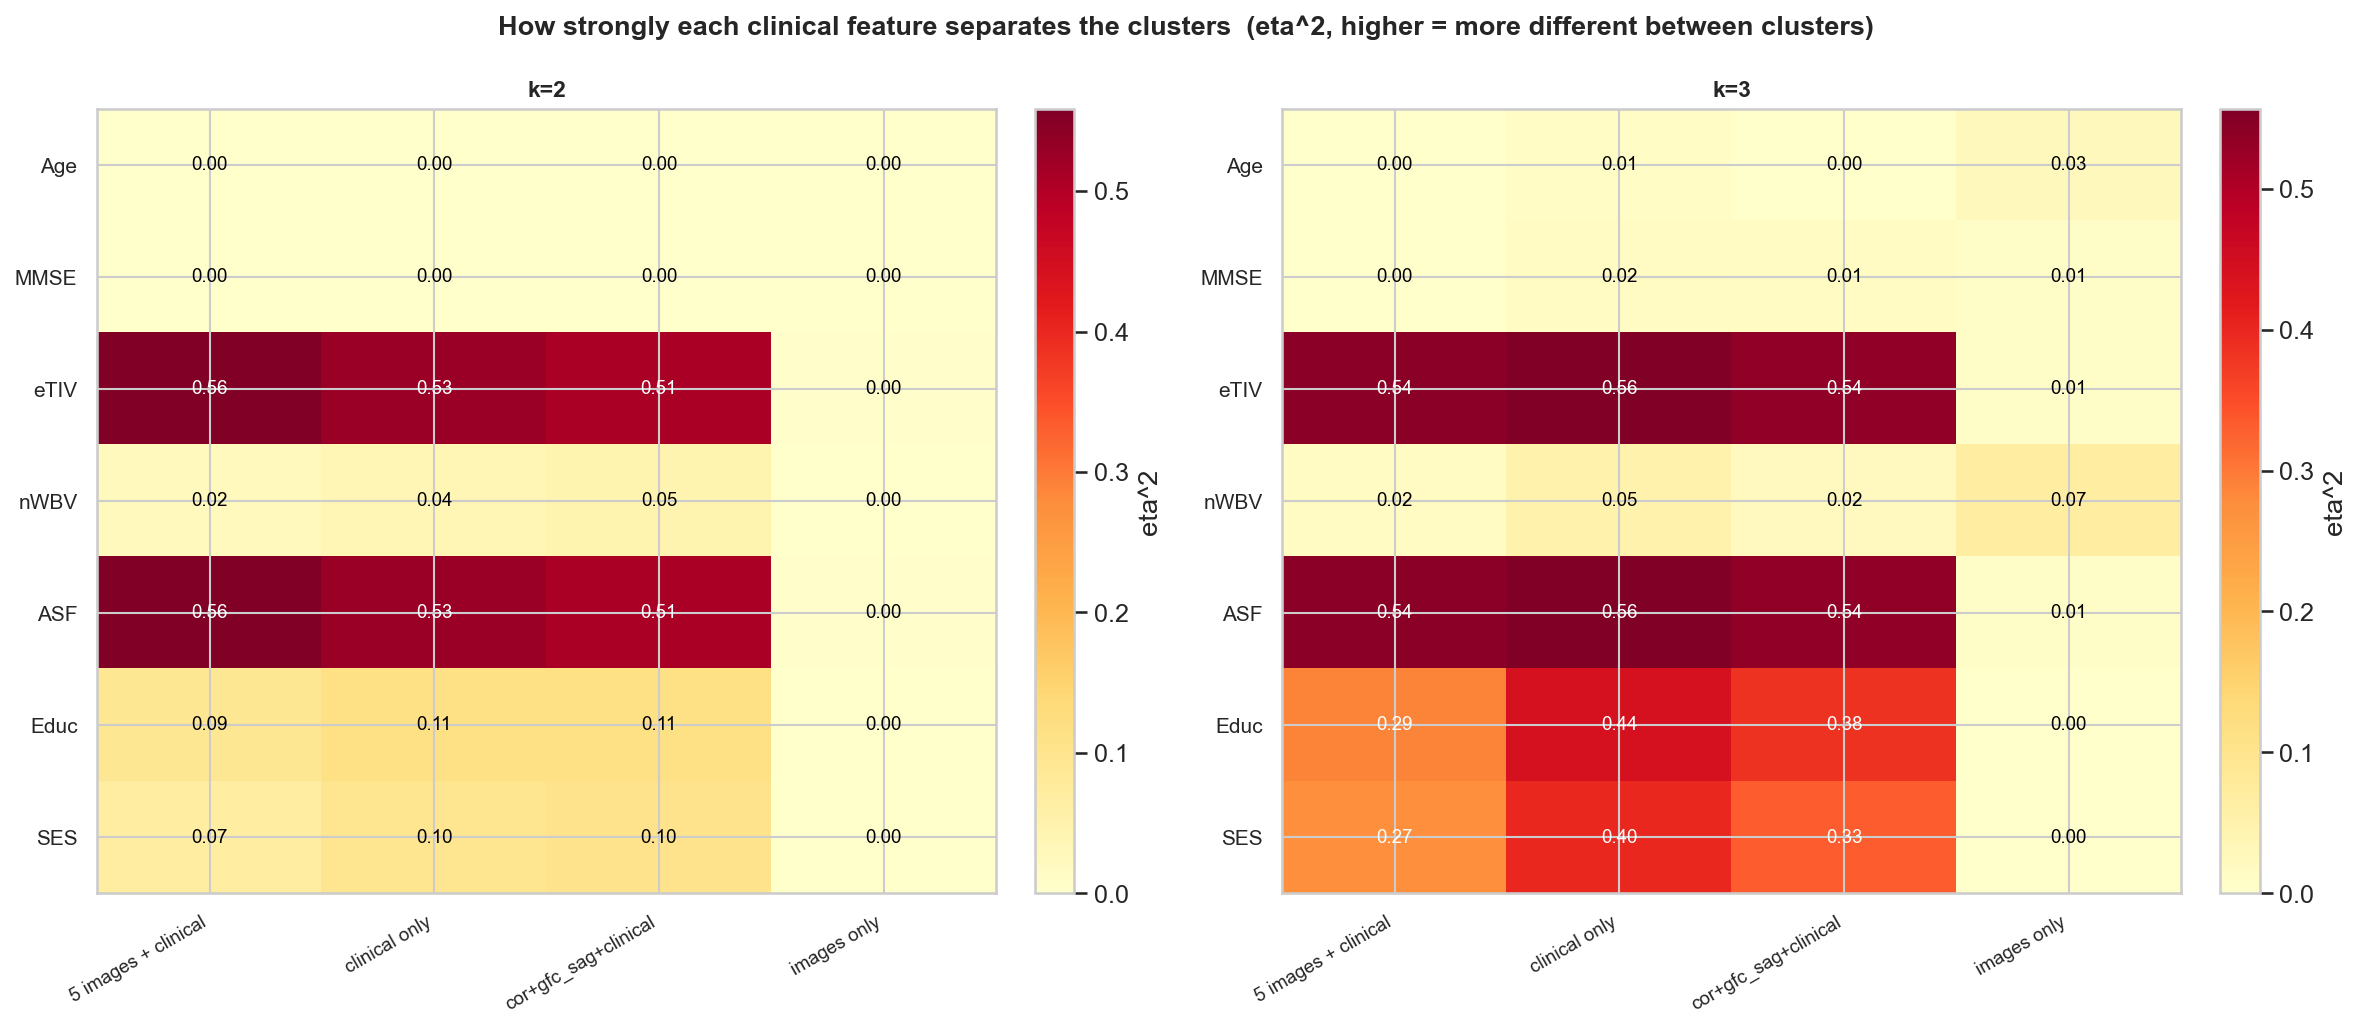
\includegraphics[width=\textwidth]{feature_separation_eta2.png}
    \caption{Effect size ($\eta^2$, higher = stronger separation) of each clinical feature across
    four feature-set configurations (5 images+clinical, clinical-only, best 2-image+clinical,
    images-only). eTIV and sex consistently show the largest effect sizes.}
    \label{fig:eta2}
\end{figure}

\noindent \textbf{Which features actually drive the clusters.} At $k=3$, sex shows a large effect
(Cram\'er's $V=0.560$) and eTIV/ASF a large effect ($\eta^2=0.543$/$0.542$); education and SES are
also large ($\eta^2=0.287$ and $0.273$). Age and MMSE are negligible ($\eta^2\approx0.000$), and
CDR itself (external, never used in clustering) registers only $V=0.135$. The same ordering
holds at $k=2$ (sex $V=0.642$, eTIV/ASF $\eta^2=0.558$) and across the other three configurations in
Figure~\ref{fig:eta2}. In other words, the clustering is not failing to find structure: it is
finding real, large, and highly reproducible structure, organised around sex, intracranial volume,
and socioeconomic variables, rather than around dementia severity.

\noindent \textbf{Geometric diagnostics (secondary).} Optimal-$k$ selection (elbow, silhouette,
Davies-Bouldin, $k=2$ to $8$) agrees on $k=2$ as statistically optimal, with $k=3$ also reported for
its clinical interpretability (healthy / very mild / mild--moderate); a 2D PCA scatter of the
558-column feature matrix shows PC1 alone explains $\sim$99\% of variance, so cluster boundaries
fall along a single dominant axis rather than around visually distinct groupings in 2D. These
geometric scores are reported for completeness but are secondary to the feature-level findings
above.

\noindent \textbf{Anomaly.} A second methodological anomaly, found in a related Tucker-decomposition
configuration during this same profiling phase, is worth flagging: Robust Mahalanobis at $k=3,4$
occasionally produced degenerate singleton-outlier clusters (sizes such as $\{1, 414, 1\}$) while
reporting a deceptively high silhouette score ($\sim0.78$). This is an artifact of the metric
isolating one or two extreme outliers into their own ``cluster,'' not evidence of genuine structure,
and a useful reminder that silhouette alone can be misleading whenever a partition is highly
imbalanced.

\subsection{Per-Block Distance Update (Package 0.1.27)}
\label{sec:perblock}

Partway through this project, the advisor released an update to \texttt{robust-mixed-dist} (0.1.27)
that allows \emph{different} distances for different quantitative blocks within RelMS, rather than
one distance string applied to every block. All four notebook 18 configurations (5 images +
clinical, clinical only, images only, and the best 2-image combination + clinical) were rebuilt
under the updated package, applying a single, consistent rule wherever a clinical quantitative block
exists: the image blocks remain on Euclidean distance exactly as before, and the clinical block
switches to Robust Mahalanobis distance, the professor's own example of the new capability. The
images-only configuration has no clinical block, so it is numerically unchanged from notebook 18.

\begin{figure}[H]
    \centering
    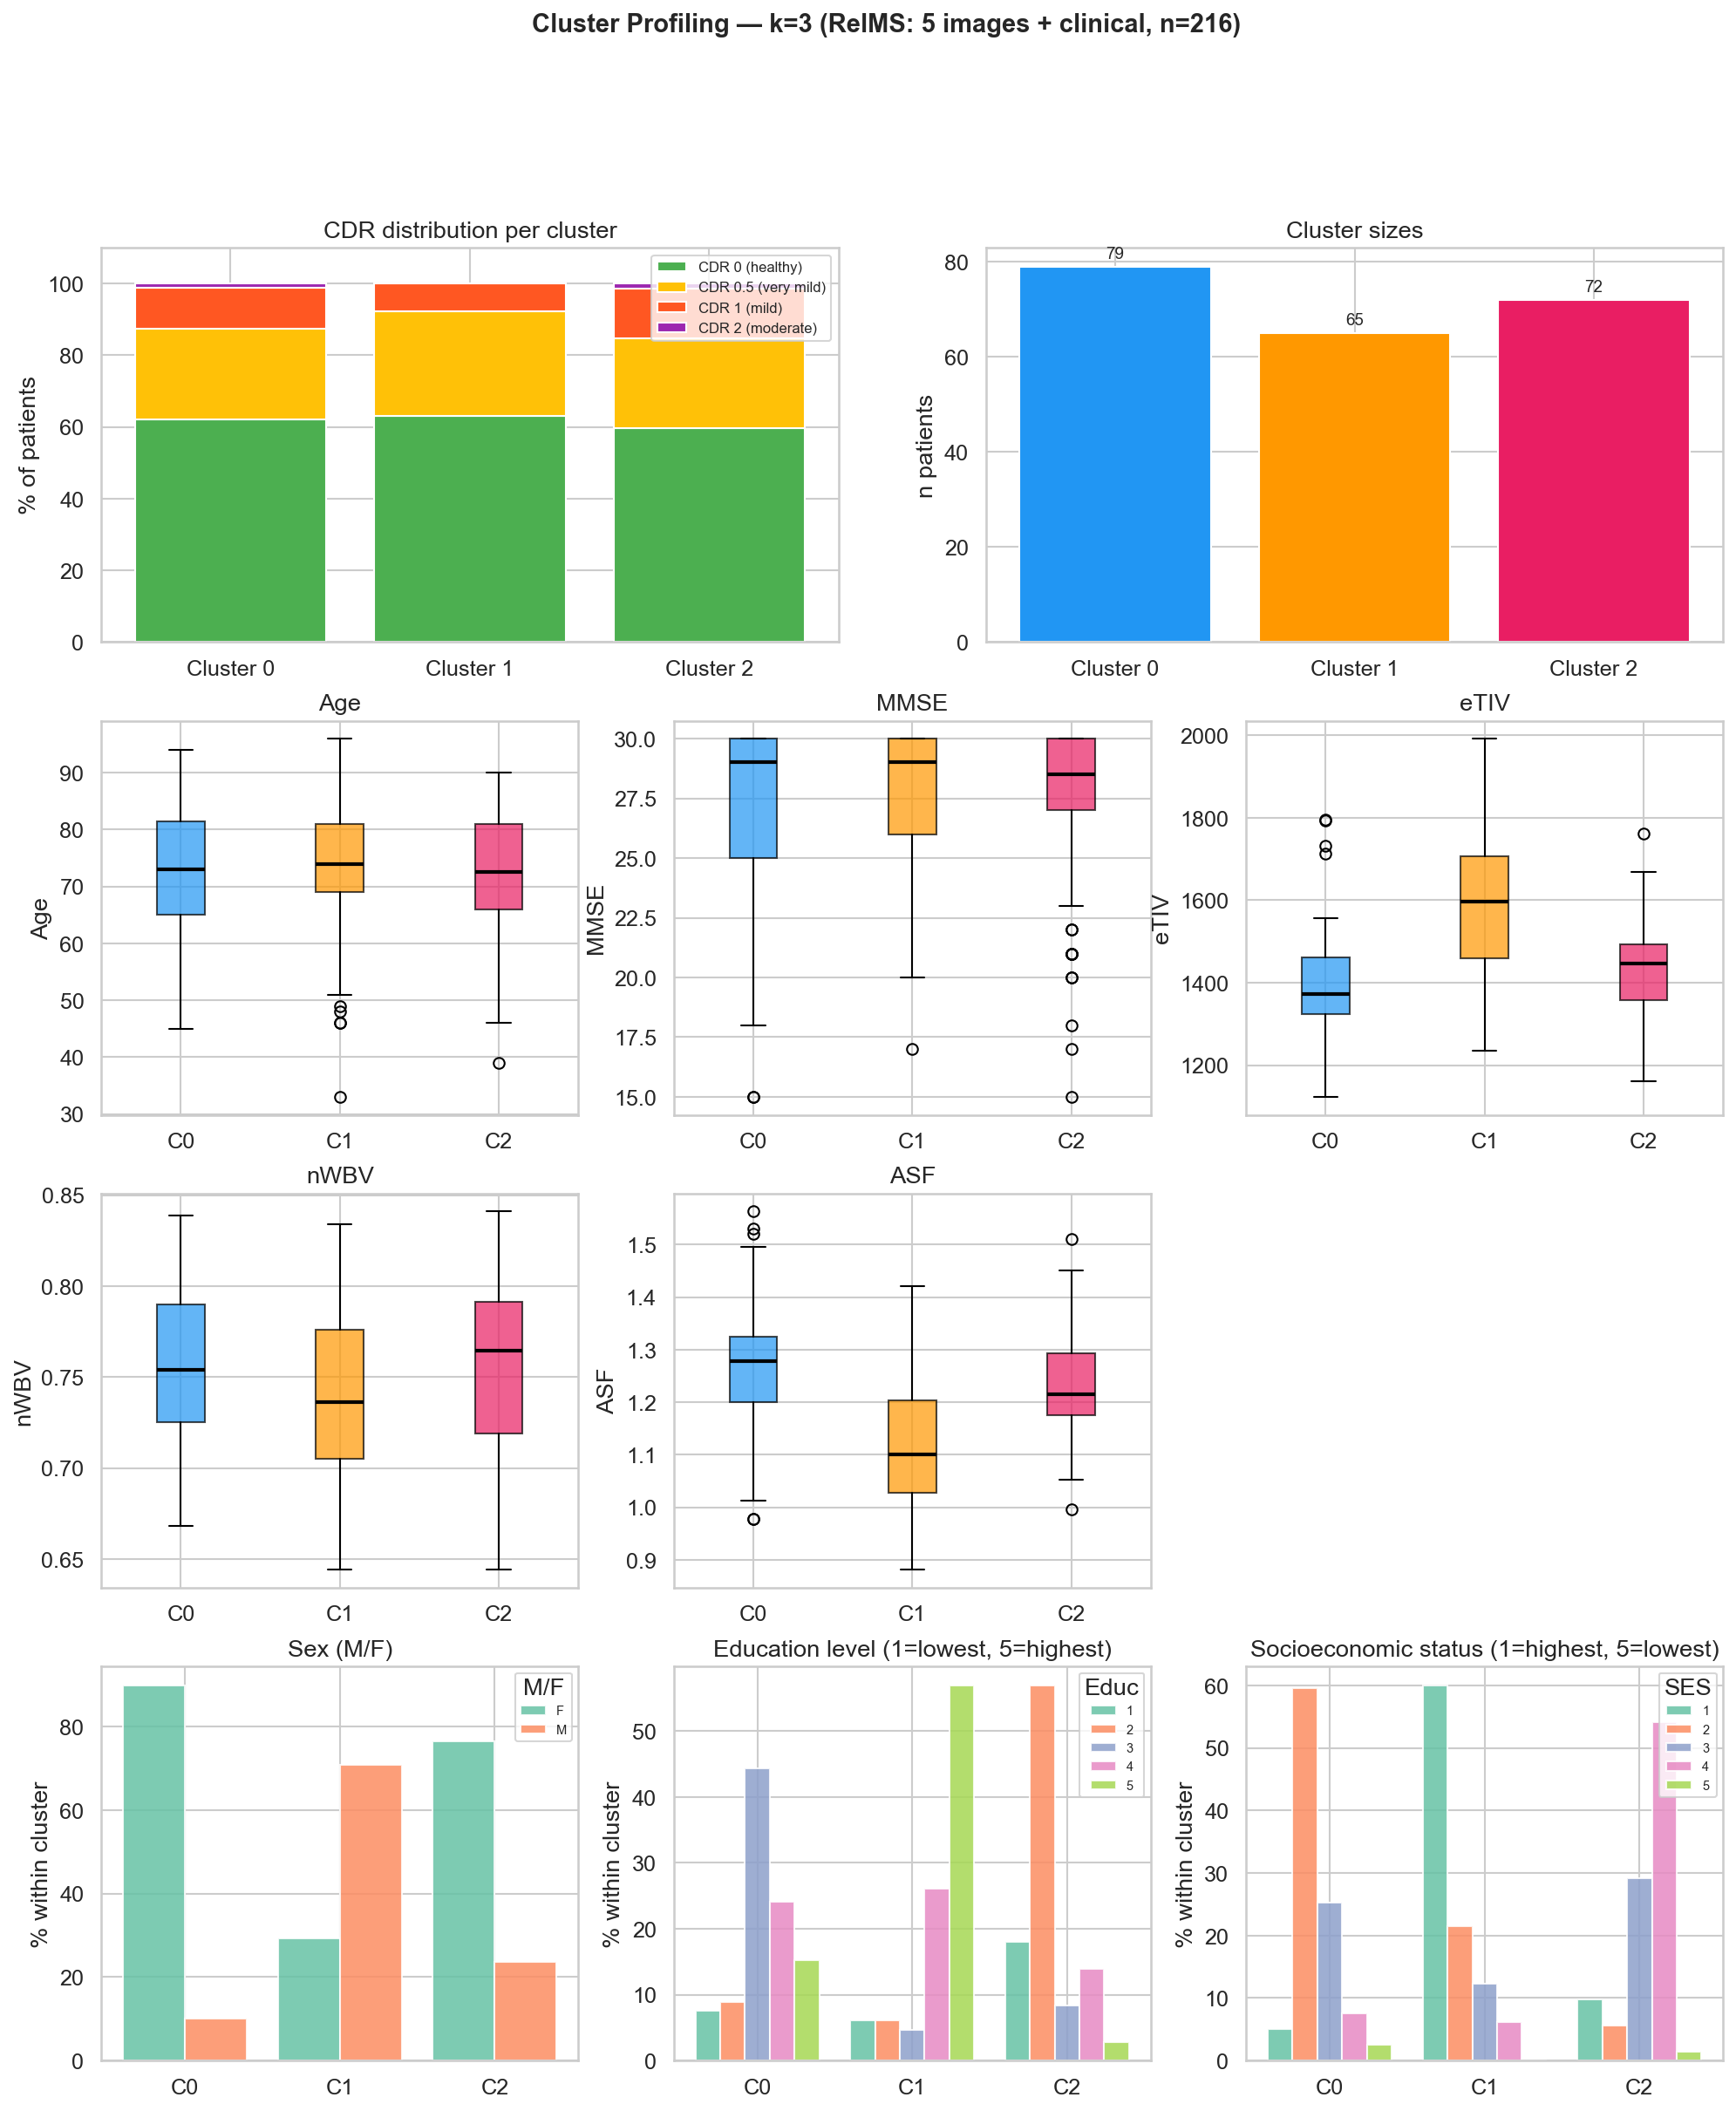
\includegraphics[width=\textwidth]{updated_cluster_profile_k3.png}
    \caption{Full cluster profile at $k=3$ under the updated (Robust-Mahalanobis-clinical-block)
    5-image+clinical configuration (the direct counterpart to Figure~\ref{fig:profilek3}). The
    same pattern holds: sex and eTIV visibly separate the clusters, CDR does not.}
    \label{fig:nb19profilek3}
\end{figure}

\begin{figure}[H]
    \centering
    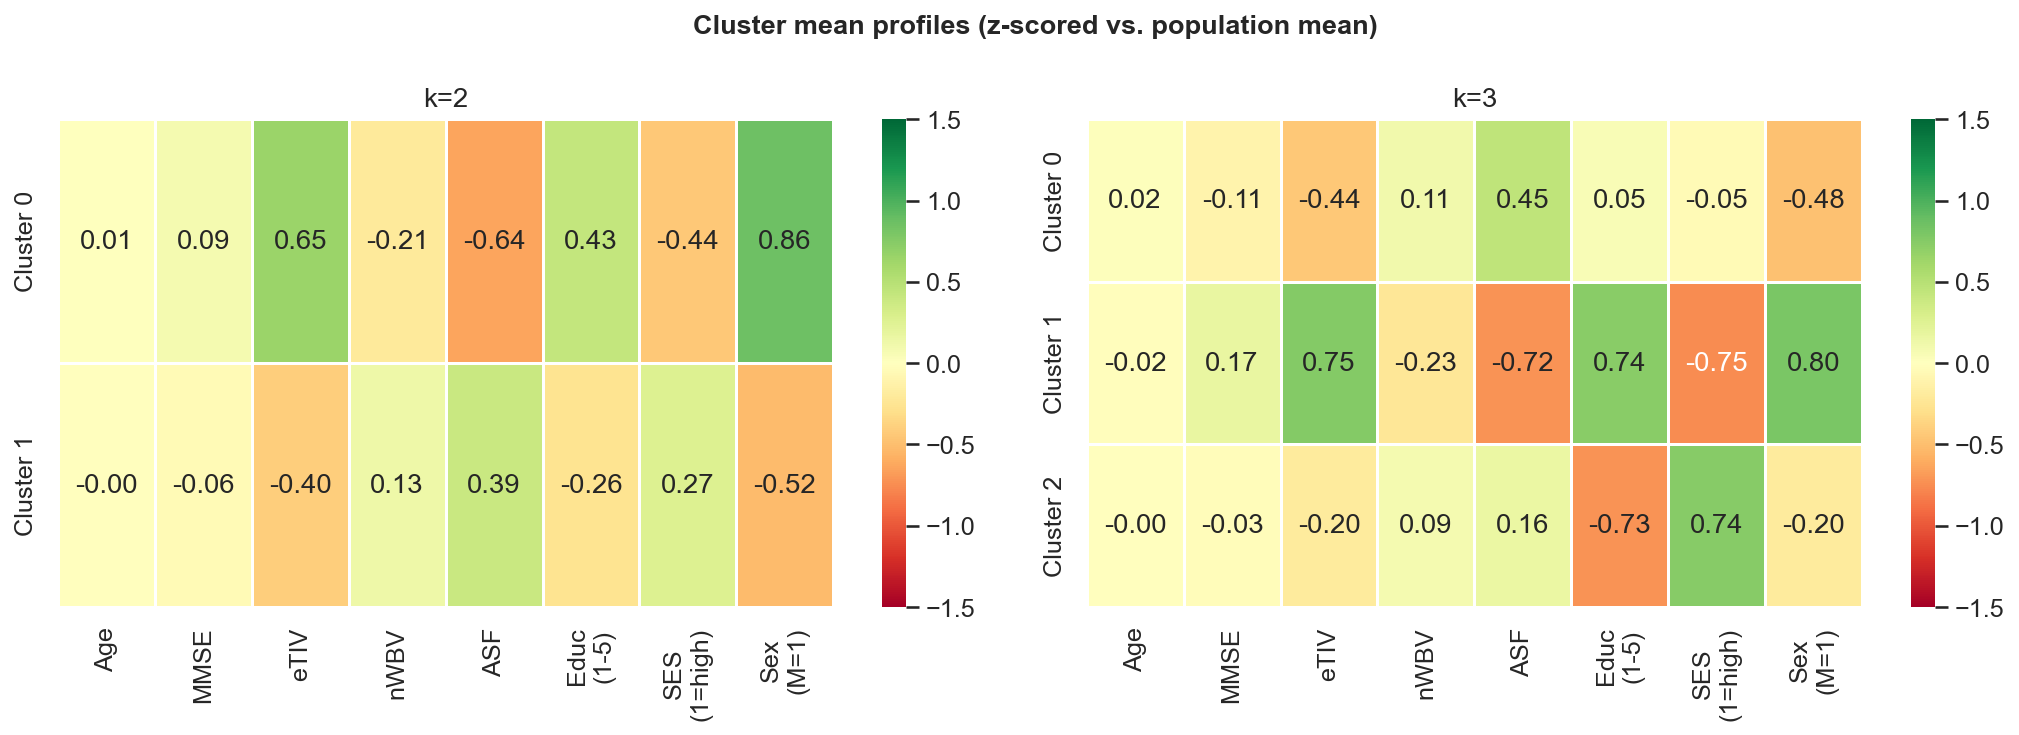
\includegraphics[width=0.85\textwidth]{updated_cluster_profile_heatmap.png}
    \caption{Cluster mean profile (z-scored), $k=2$ and $k=3$, under the updated configuration
    (the direct counterpart to Figure~\ref{fig:heatmap18}).}
    \label{fig:nb19heatmap}
\end{figure}

\begin{figure}[H]
    \centering
    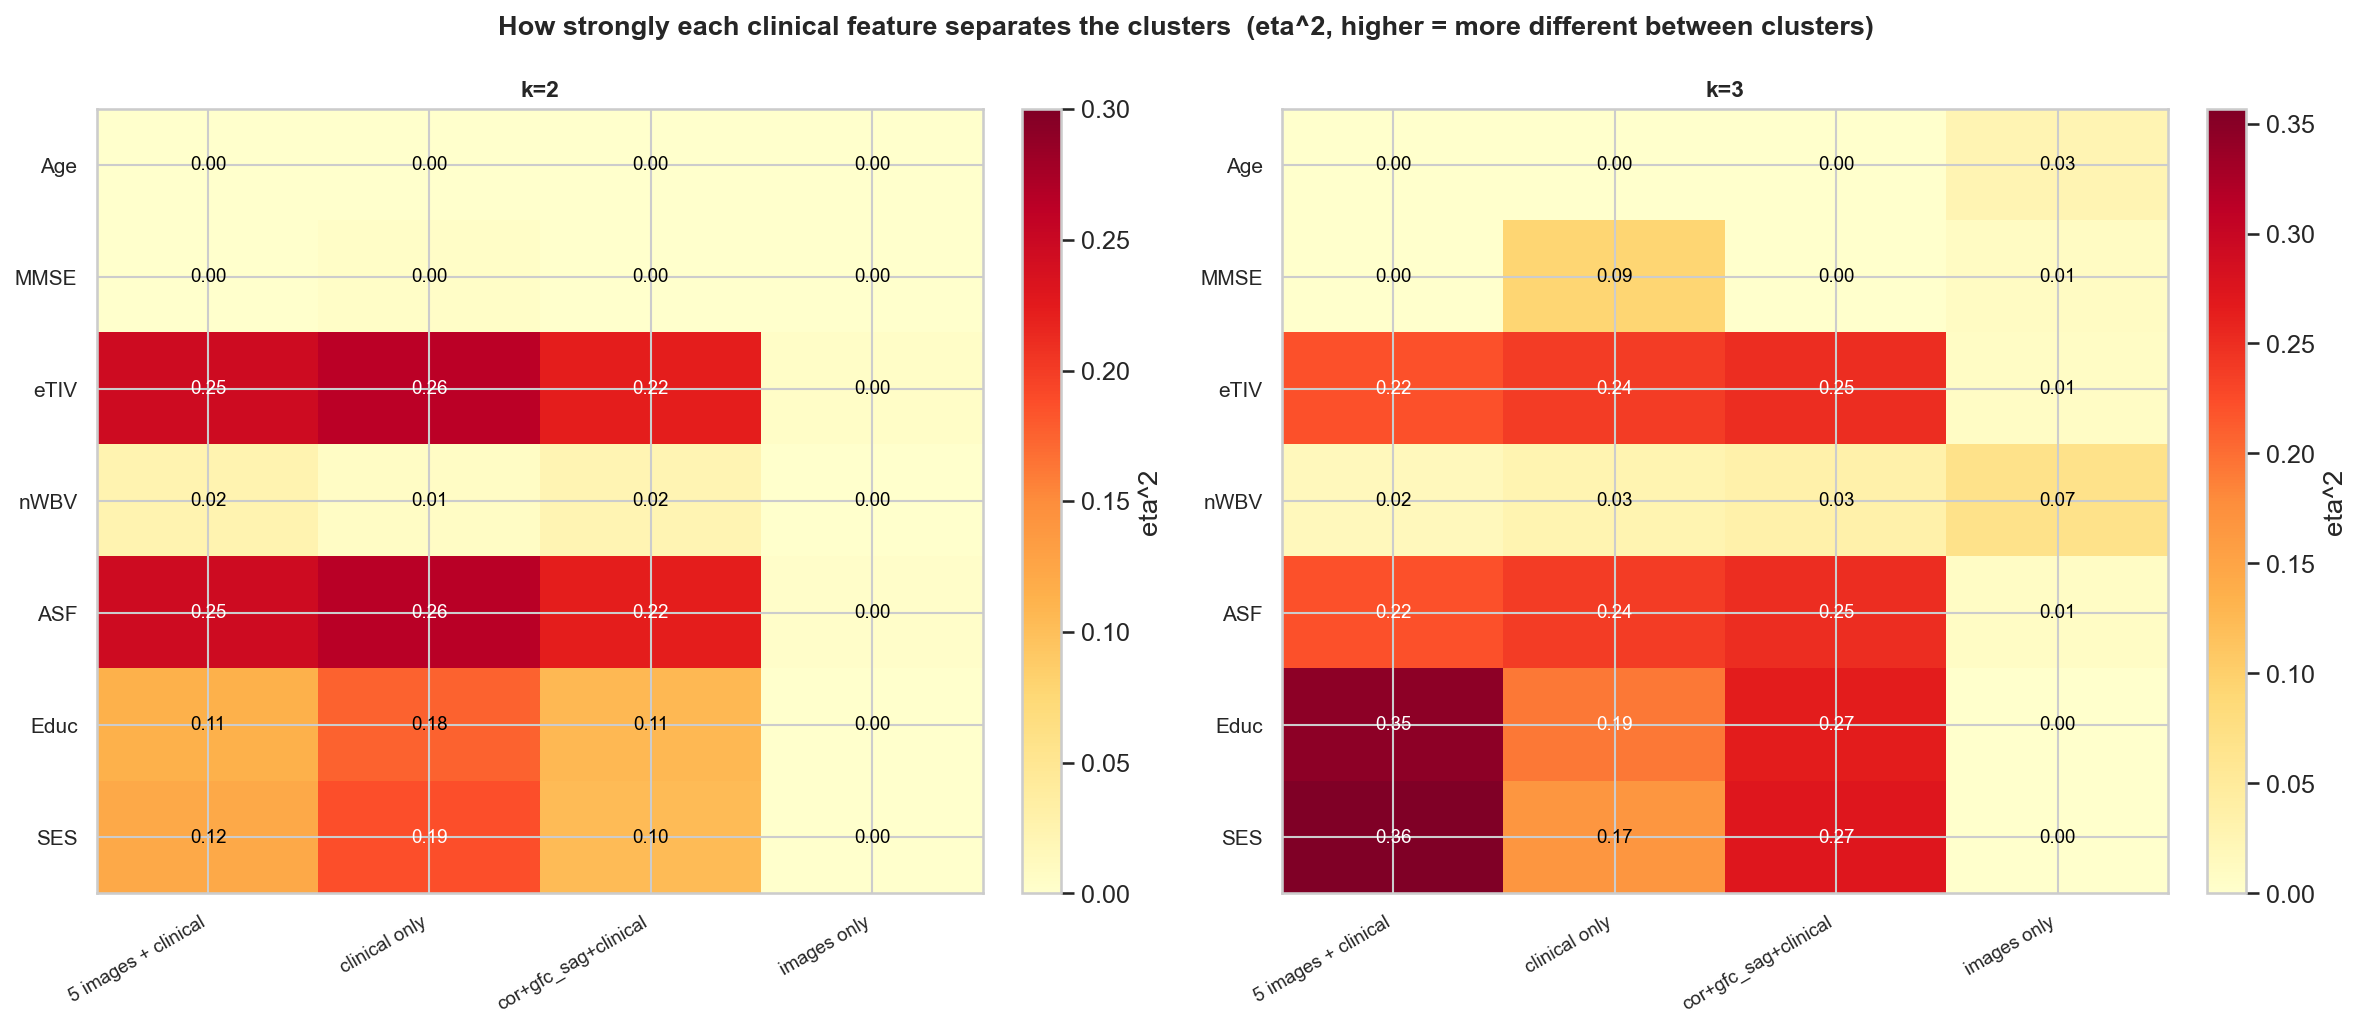
\includegraphics[width=\textwidth]{updated_feature_separation_eta2.png}
    \caption{Effect size ($\eta^2$) of each clinical feature across the four updated
    (Robust-Mahalanobis-clinical-block) configurations (the direct counterpart to
    Figure~\ref{fig:eta2}). The same features (sex, eTIV) dominate as under the original Euclidean
    setup.}
    \label{fig:nb19eta2}
\end{figure}

\noindent \textbf{Feature separation is preserved under the update.} The same large, reproducible
effects seen in Section~\ref{sec:flagship} persist here: sex and eTIV/ASF remain the dominant
differentiators in every one of the four updated configurations, at essentially the same magnitude
as under plain Euclidean (compare Figure~\ref{fig:nb19eta2} to Figure~\ref{fig:eta2}). Switching the
clinical block's distance function changes \emph{which patients} fall into each cluster (see the
geometric comparison below), but not \emph{what kind} of structure the clustering finds overall.

\noindent \textbf{Geometric diagnostics (secondary).} Switching the clinical block to Robust
Mahalanobis made three of the four configurations slightly worse by silhouette/ARI against CDR and
left the fourth (images-only) unchanged; only clinical-only at $k=3$ improved, and by an amount (ARI
$0.018 \to 0.038$) too small to read as a real effect.

\begin{table}[H]
\centering
\footnotesize
\caption{All four notebook 18 configurations, before (Euclidean throughout) and after (clinical
block switched to Robust Mahalanobis) the package update. Images-only is identical in both columns
by construction, since it has no clinical block. Reported for completeness; see the feature-level
discussion above for the more informative comparison.}
\begin{tabular}{lccccc}
\toprule
\textbf{Configuration} & $k$ & \textbf{Sil.\ (old)} & \textbf{Sil.\ (new)} & \textbf{ARI (old)} & \textbf{ARI (new)} \\
\midrule
5 images + clinical        & 2 & 0.0262 & 0.0098 & 0.0283  & 0.0043 \\
5 images + clinical        & 3 & 0.0091 & 0.0053 & 0.0176  & -0.0063 \\
Clinical only               & 2 & 0.0292 & 0.0118 & 0.0245  & -0.0056 \\
Clinical only               & 3 & 0.0130 & 0.0064 & 0.0177  & 0.0384 \\
Images only (unchanged)     & 2 & 0.0510 & 0.0510 & -0.0040 & -0.0040 \\
Images only (unchanged)     & 3 & 0.0376 & 0.0376 & -0.0205 & -0.0205 \\
Best combo + clinical       & 2 & 0.0269 & 0.0109 & 0.0320  & 0.0058 \\
Best combo + clinical       & 3 & 0.0112 & 0.0065 & 0.0161  & -0.0045 \\
\bottomrule
\end{tabular}
\end{table}

\noindent Diagnosing the small CDR movements above required looking at the clinical variables
themselves: \texttt{eTIV} and
\texttt{ASF} are correlated at $r=-0.990$ in this cohort (ASF is computed as an atlas scaling factor
derived from head size, so the two are near-mathematical duplicates), making the clinical block's
$5\times5$ correlation matrix nearly singular (smallest eigenvalue $0.010$ vs.\ largest $2.262$,
condition number $\approx 218$). Robust Mahalanobis distance inverts that correlation structure,
which amplifies estimation noise along the near-degenerate \texttt{eTIV}/\texttt{ASF} direction.
Euclidean distance, which never inverts anything, is not exposed to this instability. A targeted
follow-up check on the clinical-only block confirmed the mechanism is real rather than arbitrary:
Robust Mahalanobis gives MMSE (the single clinical variable most directly tied to dementia severity)
roughly $5.5\times$ more influence over the resulting clusters than Euclidean does ($\eta^2=0.093$
vs.\ $0.017$ at $k=3$), which is exactly why clinical-only improved slightly at that $k$. Even so,
this extra influence is still far too small, on its own, to produce a meaningfully CDR-aligned
partition.
\textbf{The distance metric is not the bottleneck}: it can be tuned to give more weight to
clinically relevant variables, and when it does, the effect on CDR alignment is still marginal,
confirming that the limiting factor is the absence of CDR-discriminative signal in the feature set
itself rather than any particular choice of distance.

% ══════════════════════════════════════════════════════════════════════════════
\section{Discussion}
\label{sec:discussion}

\subsection{Central Finding}
Across all nine stages (single image types, merged images, Generalised Gower, RelMS, two-image
combinations, a leave-one-image-out sweep, and the post-update per-block distance comparison across
all four notebook 18 configurations), \textbf{the clustering consistently recovers real, large,
reproducible structure, but that structure is organised around sex and total intracranial volume
(eTIV/ASF), not around CDR}. The effect sizes behind this are substantial by conventional standards:
sex reaches Cram\'er's $V$ up to $0.66$ and eTIV/ASF reach $\eta^2$ up to $0.56$ across every
configuration tested (Figures~\ref{fig:eta2} and~\ref{fig:nb19eta2}), with education and SES also
registering large effects ($\eta^2$ up to $0.44$) at several configurations. Age and MMSE, by
contrast, are consistently negligible ($\eta^2\approx0.00$--$0.02$). Measured specifically against
CDR, this same structure is weak: ARI against CDR stays roughly within $[-0.02, +0.06]$ and NMI
within $[0.01, 0.10]$ throughout, i.e.\ barely above what a random partition would achieve on that
axis, and the best single CDR-aligned result across the entire project is \texttt{masked\_tra} alone,
Euclidean distance, $k=3$ (ARI $=0.060$, NMI $=0.085$). The picture that emerges is best described
as a \emph{mismatch of axes} rather than an absence of structure: HOG+PCA features recovered from
these MRI images carry a strong, stable signal about demographic and anatomical variation, and that
signal survives every distance metric, block weighting, and image combination tried in this project.
It simply is not the signal clinicians use to grade dementia severity.

\subsection{Two Flagged Anomalies}
\begin{enumerate}[leftmargin=1.4em]
    \item \textbf{Generalised Gower block dominance} (Section~\ref{sec:ggower}): every image+clinical
    variant under Generalised Gower reproduced the clinical-only baseline exactly, suggesting the
    clinical block dominated that particular distance formulation so completely that image features
    contributed no signal. This was the direct motivation for adopting RelMS, and remains worth a
    closer look at the underlying scaling interaction within the Generalised Gower implementation.
    \item \textbf{Degenerate outlier clusters under Robust Mahalanobis} (Section 4.8): in a related
    Tucker-decomposition configuration, Robust Mahalanobis occasionally isolated 1--2 extreme
    outliers into their own cluster while reporting an artificially high silhouette score, a
    caution against trusting silhouette alone without checking cluster-size balance.
\end{enumerate}


% ══════════════════════════════════════════════════════════════════════════════
\section{Conclusion}

This project built a full pipeline (HOG feature extraction, per-image PCA, and a systematic
sweep across Robust Mahalanobis, Generalised Gower, and RelMS distance metrics, single- and
multi-image feature combinations, and, most recently, per-block distance-function sensitivity)
to test whether brain MRI structure, with or without standard clinical variables, can recover
Alzheimer's disease severity groups in an unsupervised setting. The clustering itself works well:
every configuration tested recovers clusters with large, consistent, and reproducible separation on
sex (Cram\'er's $V$ up to $0.66$) and total intracranial volume (eTIV/ASF, $\eta^2$ up to $0.56$),
and several configurations also separate cleanly on education and SES. What those clusters do not
do, consistently, is line up with CDR. The strongest single CDR-aligned result
(\texttt{masked\_tra}, Euclidean, $k=3$, ARI~$=0.060$) and the redundancy/leave-one-out analyses
point toward \texttt{masked\_tra} and \texttt{sbj\_sag} as the most anatomically distinctive image
types, while the effect-size analysis points toward sex and intracranial volume, rather than
CDR-adjacent variables, as the strongest drivers of the structure actually recovered. Two
methodological anomalies were documented rather than silently resolved, for future investigation.
Overall, this is a well-controlled result that narrows the problem rather than leaving it open. The
bottleneck is not the choice of distance metric, block weighting, or image combination (all of
those reliably find real structure), but the absence, in this particular image representation, of
a signal that happens to align with dementia severity specifically.

\end{document}
